\documentclass[cn,11pt]{elegantbook}

\title{ElegantBook:优美的 \LaTeX{} 书籍模板}
\subtitle{Elegant\LaTeX{} 经典之作}

\author{Ethan Deng \& Liam Huang}
\institute{Elegant\LaTeX{} Program}
\date{\today}
\version{3.09}

\extrainfo{Victory won\rq t come to us unless we go to it. --- M. Moore}

\logo{logo.png}
\cover{cover.jpg}

\begin{document}

\maketitle

\tableofcontents
% \thispagestyle{empty}

\mainmatter
\hypersetup{pageanchor=true}

\chapter{Elegant\LaTeX{} 系列模板介绍}


Elegant\LaTeX{} 项目组致力于打造一系列美观、优雅、简便的模板方便用户使用。目前由 \href{https://github.com/ElegantLaTeX/ElegantNote}{ElegantNote},\href{https://github.com/ElegantLaTeX/ElegantBook}{ElegantBook},\href{https://github.com/ElegantLaTeX/ElegantPaper}{ElegantPaper} 组成,分别用于排版笔记,书籍和工作论文。强烈推荐使用最新正式版本!本文将介绍本模板的一些设置内容以及基本使用方法。如果您有其他问题,建议或者意见,欢迎在 Github 上给我们提交 \href{https://github.com/ElegantLaTeX/ElegantBook/issues}{issues} 或者邮件联系我们。


我们的联系方式:
\begin{itemize}
\item 官网:\href{https://elegantlatex.org/}{https://elegantlatex.org/}
\item Github 网址:\href{https://github.com/ElegantLaTeX/}{https://github.com/ElegantLaTeX/}
\item CTAN 地址:\href{https://ctan.org/pkg/elegantbook}{https://ctan.org/pkg/elegantbook}
\item 文档 Wiki:\href{https://github.com/ElegantLaTeX/ElegantBook/wiki}{https://github.com/ElegantLaTeX/ElegantBook/wiki}
\item 下载地址:\href{https://github.com/ElegantLaTeX/ElegantBook/releases}{正式发行版},\href{https://github.com/ElegantLaTeX/ElegantBook/archive/master.zip}{最新版}
\item 微博:ElegantLaTeX
\item 微信公众号:ElegantLaTeX
\item 用户 QQ 群:692108391 
\item 邮件:\email{elegantlatex2e@gmail.com}
\end{itemize}


\section{ElegantBook 更新说明}

此次更新主要有
\begin{enumerate}
\item 删除 \lstinline{\elegantpar} 命令;
\item 修复符号字体设置;
\item 增加双栏目录选项;
\item 修改脚注格式;
\item 其他。
\end{enumerate}

\begin{note}
2.x 版本的用户请仔细查看\href{https://github.com/ElegantLaTeX/ElegantBook/wiki/convert}{跨版本转换}。
\end{note}

\section{模板安装与更新}
你可以通过免安装的方式使用本模板,也可以通过安装模板的方式使用。

免安装使用方法如下,从 Github 或者 CTAN 下载最新(正式)版文件,严格意义上只需要类文件 \lstinline{elegantbook.cls}。然后将模板文件放在你的工作目录下即可使用。这样使用的好处是,无需安装,简便;缺点是,当模板进行更新之后,你需要手动替换 \lstinline{cls} 文件。

如果你是 \TeX{} Live 2019 用户,我们非常推荐你直接进行安装和更新。你可以通过 \TeX{} Live 2019 自带的 \lstinline{tlshell}\footnote{也叫 \TeX{} Live Manager} 进行安装。安装非常简单,步骤如下,搜索并打开 \lstinline{tlshell},然后通过 \lstinline{File -> Load Default Repository} 加载远程仓库,如果你不想使用默认的仓库,你可以通过 \lstinline{Options} 下的菜单设置远程仓库。设置好仓库之后,等待仓库加载完毕,你可以在下面的搜索栏搜索 \lstinline{elegantbook},然后选择进行安装与更新。

\begin{figure}[htbp]
\centering
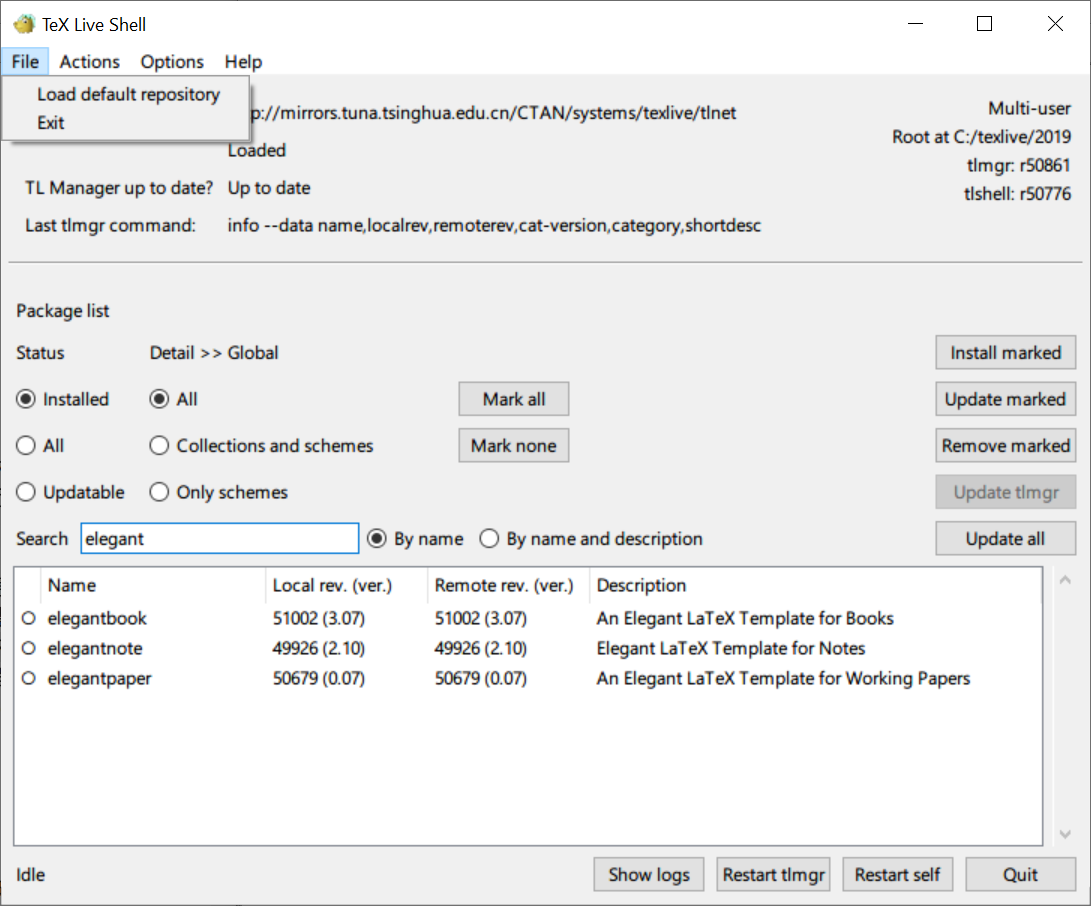
\includegraphics[width=0.7\textwidth]{tlshell.png}
\caption{使用 \TeX{} Live Shell 安装 ElegantBook 模板}
\end{figure}

如果你是 \TeX{} Live 2018 的用户,由于 2018 无法直接更新到 2019,所以你想更新的话,需要卸载 2018 重装 2019。如果你实在不想折腾,那么你仍然可以使用本模板。你可以手动安装模板,将 \lstinline{elegantbook.cls} 复制到你的 \TeX{} Live 目录下,默认安装目录为 \lstinline|C:\texlive\2019\texmf-dist\tex\latex\elegantbook|,然后通过命令行(管理员权限),运行 \lstinline{texhash} 即可。

啥?你是 C\TeX{} 用户?Sorry,本模板不提供支持。

更多关于 \TeX{} Live 2019 的安装使用以及 C\TeX{} 与 \TeX{} Live 的兼容、系统路径问题,请参考官方文档以及啸行的\href{https://github.com/OsbertWang/install_latex/releases}{一份简短的安装 \LaTeX{} 的介绍}。

\section{在线使用模板}
我们把三套模板全部上传到 \href{https://www.overleaf.com/}{Overleaf} 上了,网络便利的用户可以直接通过 Overleaf 在线使用我们的模板。使用 Overleaf 的好处是无需安装 \TeX{} Live 2019,可以随时随地访问自己的文件。查找模板,请在 Overleaf 模板库里面搜索 \lstinline{elegantlatex} 即可,你也可以直接访问\href{https://www.overleaf.com/latex/templates?addsearch=elegantlatex}{搜索结果}。选择适当的模板之后,将其 \lstinline{Open as Template},即可把模板存到自己账户下,然后可以自由编辑以及与别人一起协作。更多关于 Overleaf 的介绍和使用,请参考 Overleaf 的\href{https://www.overleaf.com/learn}{官方文档}。

\begin{remark}
Overleaf 上,中文需要使用 \lstinline{XeLaTeX} 进行编译,英文可以使用 \lstinline{PDFLaTeX} 与 \lstinline{XeLaTeX} 进行编译。
\end{remark}

\section{用户作品计划}
Elegant\LaTeX{} 系列模板从创立至今已经有 8 年了,我们的模板也受到了很多用户的喜爱,在此,为了促进模板用户之间的交流,了解用户需求,完善本模板,我们将建立一个区域专门展示用户的文档,包括但不限于 Github 和官网等。如果你愿意将自己的作品展示出来,请邮件或者其他方式联系我们。如果自己代码已经传到 Github 或者 Gitee 等网站,可以提供对应网址。


\centerline{\textcolor{red}{\bfseries 广告位招租!}}

\section{关于提交}
出于某些因素的考虑,Elegant\LaTeX{} 项目自 2019 年 5 月 20 日开始,\textbf{不再接受任何非作者预约性质的提交}(pull request)!如果你想改进模板,你可以给我们提交 issues,或者可以在遵循协议(LPPL-1.3c)的情况下,克隆到自己仓库下进行修改。

\section{协作人员招募}
招募 Elegant\LaTeX{} 的协作人员,没有工资。工作内容:翻译 Elegant\LaTeX{} 系列模板相关的文稿(中文->英文),维护模板的 wiki(主要涉及 Markdown 语法),如果有公众号文稿写作经历的话,也可以帮忙写微信稿。本公告长期有效。

目前 ElegantLaTeX 共有 4 名协作人员,分别是
\begin{itemize}
	\item 官方文档翻译: \href{https://github.com/peggy2006xzyz}{YPY};
	\item Github 维基维护: \href{https://github.com/izinngo}{Ingo Zinngo}、\href{https://github.com/xiaohao890809}{追寻原风景};
	\item QQ 群管理员: \href{https://github.com/sikouhjw}{Sikouhjw}.
\end{itemize}

在此感谢他们无私的奉献!

\section{致谢}
2019 年 5 月 20 日,ElegantBook 模板在 Github 上的收藏数(star)达到了 100\footnote{截止 2019 年 8 月 18 日 3.09 版本正式发布,star 数为 189。}。

在此特别感谢 China\TeX{} 以及 \href{http://www.latexstudio.net/}{\LaTeX{} 工作室}对于本系列模板的大力宣传与推广。\LaTeX{} 工作室网站上有很多精彩的帖子和精致的模板,欢迎大家去挖掘里面的宝藏。这也是国内最全面的 \LaTeX{} 相关的网站。也非常感谢 \href{https://github.com/muzimuzhi}{muzimuzhi} 对于模板的完善。

如果你喜欢我们的模板,你可以在 Github 上收藏我们的模板。
\begin{figure}[htbp]
\centering
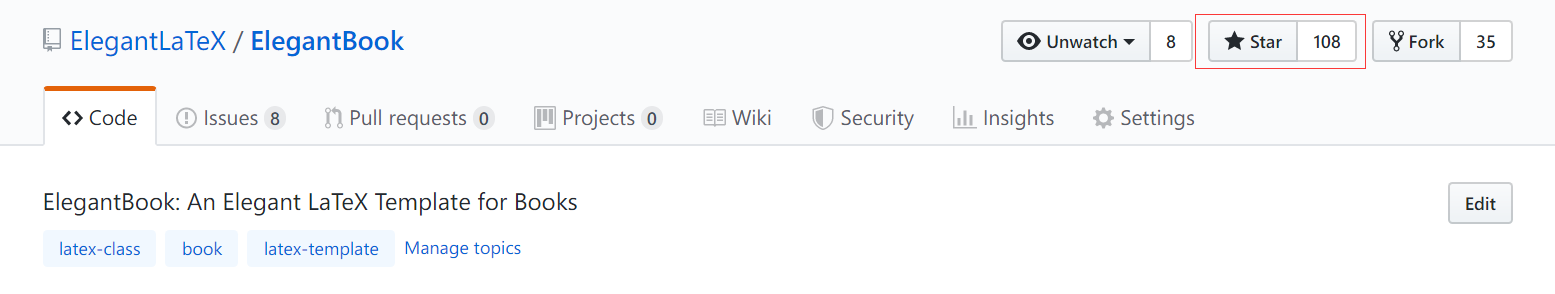
\includegraphics[width=\textwidth]{star.png}
\caption{一键三连求赞}
\end{figure}

\begin{figure}[htbp]
\centering
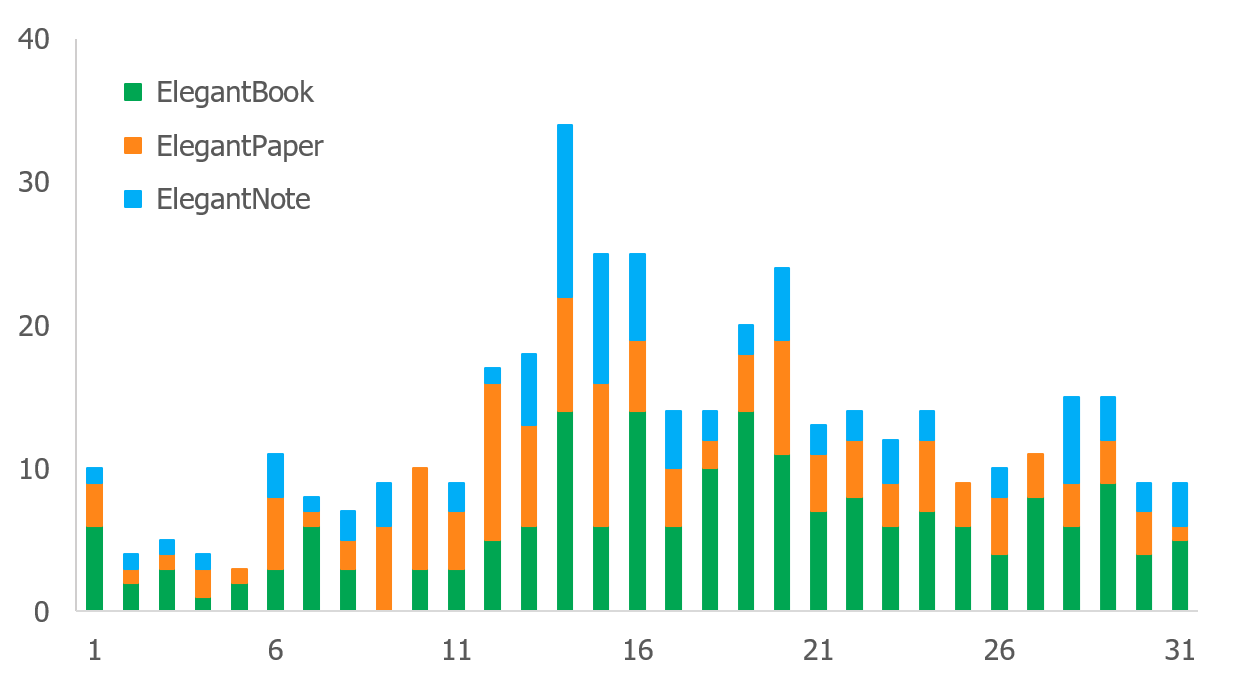
\includegraphics[width=0.618\textwidth]{star-history.png}
\caption{Elegant\LaTeX{} 系列模板上线 Github 之后上每周 Star 数变化}
\end{figure}

\section{捐赠}
如果您非常喜爱我们的模板或者我,你还可以选择捐赠以表达您对我们模板和我的支持。本模板自 3.08 版本发布了捐赠信息之后,收到了近千元的捐赠(四舍五入就是一个亿),非常感谢!

\begin{figure}[htbp]
\centering

\includegraphics[width=0.5\textwidth]{donate.jpg}
\end{figure}

\textbf{赞赏费用的使用解释权归 Elegant\LaTeX{} 所有,并且不接受监督,请自愿理性打赏}。10 元以上的赞赏,我们将列入捐赠榜,谢谢各位金主!

\begin{table}[!htbp]
  \centering
  \caption{捐赠榜}
    \begin{tabular}{crcc}
    \toprule
    捐赠者   & 金额 & 时间 & 渠道 \\
    \midrule
    Lerh  & 10 元  & 2019/05/15 & 微信 \\
    越过地平线 & 10 元    & 2019/05/15 & 微信 \\
	大熊 &  20 元 & 2019/05/27 & 微信 \\
	佚名 & 10 元 & 2019/05/30 & 微信\\
	\href{http://www.latexstudio.net/}{latexstudio.net} & 666 元 & 2019/06/05 & 支付宝\\
	Cassis & 11 元 & 2019/06/30 & 微信\\
	佚名 & 10 元 & 2019/07/23 & 微信\\
    \bottomrule
    \end{tabular}%
\end{table}%


\chapter{ElegantBook 设置说明}
本模板基于基础的 book 文类,所以 book 的选项对于本模板也是有效的(纸张无效,因为模板有设备选项)。默认编码为 UTF-8,推荐使用 \TeX{} Live 编译。本文编写环境为 Win10 (64bit) + \TeX{} Live 2019,支持 \lstinline{PDFLaTeX} 以及 \lstinline{XeLaTeX} 编译。


\section{语言模式}
本模板内含两套语言环境,改变语言环境会改变图表标题的引导词(图,表),文章结构词(比如目录,参考文献等),以及定理环境中的引导词(比如定理,引理等)。不同语言模式的启用如下:
\begin{lstlisting}
\documentclass[cn]{elegantbook} 
\documentclass[lang=cn]{elegantbook}
\end{lstlisting}

\begin{remark}
只有中文环境(\lstinline{lang=cn})才可以输入中文。另外如果抄录环境(\lstinline{lstlisting})中有中文字符,请务必使用 \lstinline{XeLaTeX} 编译。
\end{remark}

\section{设备选项}
最早我们在 ElegantNote 模板中加入了设备选项(\lstinline{device}),后来,我们觉得这个设备选项的设置可以应用到 ElegantBook 中\footnote{不过因为 ElegantBook 模板封面图片的存在,在修改页面设计时,需要对图片进行裁剪。},而且 Book 一般内容比较多,如果在 iPad 上看无需切边,放大,那用户的阅读体验将会得到巨大提升。你可以使用下面的选项将版面设置为 iPad 设备模式\footnote{默认为 normal 模式,也即 A4 纸张大小。}
\begin{lstlisting}
\documentclass[pad]{elegantbook} %or
\documentclass[device=pad]{elegantbook}
\end{lstlisting}

\section{颜色主题}
本模板内置 5 组颜色主题,分别为 \textcolor{structure1}{\lstinline{green}}\footnote{为原先默认主题。}、\textcolor{structure2}{\lstinline{cyan}}、\textcolor{structure3}{\lstinline{blue}}(默认)、\textcolor{structure4}{\lstinline{gray}}、\textcolor{structure5}{\lstinline{black}}。另外还有一个自定义的选项  \lstinline{nocolor}。调用颜色主题 \lstinline{green} 的方法为 
\begin{lstlisting}
\documentclass[green]{elegantbook} %or
\documentclass[color=green]{elegantbook}
\end{lstlisting}

\begin{table}[htbp]
\caption{ElegantBook 模板中的颜色主题\label{tab:color thm}}
\centering
\begin{tabular}{ccccccc}
\toprule
	        & \textcolor{structure1}{green} 
	        & \textcolor{structure2}{cyan} 
	        & \textcolor{structure3}{blue}
	        & \textcolor{structure4}{gray} 
	        & \textcolor{structure5}{black} 
	        & 主要使用的环境\\
\midrule
structure & \makecell{{\color{structure1}\rule{1cm}{1cm}}}
				& \makecell{{\color{structure2}\rule{1cm}{1cm}}}
				& \makecell{{\color{structure3}\rule{1cm}{1cm}}} 
				& \makecell{{\color{structure4}\rule{1cm}{1cm}}} 
				& \makecell{{\color{structure5}\rule{1cm}{1cm}}} 
				& chapter \ section \ subsection \\

main      & \makecell{{\color{main1}\rule{1cm}{1cm}}}
				& \makecell{{\color{main2}\rule{1cm}{1cm}}}
				& \makecell{{\color{main3}\rule{1cm}{1cm}}}
				& \makecell{{\color{main4}\rule{1cm}{1cm}}}
				& \makecell{{\color{main5}\rule{1cm}{1cm}}}
				& definition \ exercise \ problem \\

second    & \makecell{{\color{second1}\rule{1cm}{1cm}}}
				& \makecell{{\color{second2}\rule{1cm}{1cm}}}
				& \makecell{{\color{second3}\rule{1cm}{1cm}}}
				& \makecell{{\color{second4}\rule{1cm}{1cm}}}
				& \makecell{{\color{second5}\rule{1cm}{1cm}}}
				& theorem \ lemma \ corollary\\

third     & \makecell{{\color{third1}\rule{1cm}{1cm}}}
				& \makecell{{\color{third2}\rule{1cm}{1cm}}}
				& \makecell{{\color{third3}\rule{1cm}{1cm}}}
				& \makecell{{\color{third4}\rule{1cm}{1cm}}}
				& \makecell{{\color{third5}\rule{1cm}{1cm}}}
				& proposition\\
\bottomrule
\end{tabular}
\end{table}

如果需要自定义颜色的话请选择 \lstinline{nocolor} 选项或者使用 \lstinline{color=none},然后在导言区定义 structurecolor、main、second、third 颜色,具体方法如下:
\begin{lstlisting}
\definecolor{structurecolor}{RGB}{0,0,0}
\definecolor{main}{RGB}{70,70,70}    
\definecolor{second}{RGB}{115,45,2}    
\definecolor{third}{RGB}{0,80,80}   
\end{lstlisting}


\section{章标题显示风格}

本模板内置 2 套\textit{章标题显示风格},包含 \lstinline{hang}(默认)与 \lstinline{display} 两种风格,区别在于章标题单行显示(\lstinline{hang})与双行显示(\lstinline{display}),本说明使用了 \lstinline{hang}。调用方式为
\begin{lstlisting}
\documentclass[hang]{elegantbook} %or
\documentclass[titlestyle=hang]{elegantbook}
\end{lstlisting}

\section{数学环境简介}

在我们这个模板中,我们定义了两种不同的定理模式 \lstinline{mode},包括简单模式(\lstinline{simple})和炫彩模式(\lstinline{fancy}),默认为 \lstinline{fancy} 模式,不同模式的选择为
\begin{lstlisting}
\documentclass[simple]{elegantbook} %or
\documentclass[mode=simple]{elegantbook}
\end{lstlisting}

本模板定义了四大类环境

\begin{itemize}
\item \textit{定理类环境},包含标题和内容两部分,全部定理类环境的编号均以章节编号。根据格式的不同分为 3 种
   \begin{itemize}
      \item \textcolor{main}{\textbf{definition}} 环境,颜色为 \textcolor{main}{main};
      \item \textcolor{second}{\textbf{theorem、lemma、corollary}} 环境,颜色为 \textcolor{second} {second};
      \item \textcolor{third}{\textbf{proposition}} 环境,颜色为 \textcolor{third}{third}。
   \end{itemize}
\item \textit{示例类环境},有 \textbf{example、problem、exercise} 环境(对应于例、例题、练习),自动编号,编号以章节为单位,其中 \textbf{exercise} 有提示符。
\item \textit{提示类环境},有 \textbf{note} 环境,特点是:无编号,有引导符。
\item \textit{结论类环境},有 \textbf{conclusion、assumption、property,remark、solution} 环境\footnote{本模板还添加了一个 result 选项,用于隐藏 \lstinline{solution} 和 \lstinline{proof} 环境,默认为显示(\lstinline{result=answer}),隐藏使用 \lstinline{result=noanswer}。},三者均以粗体的引导词为开头,和普通段落格式一致。
\end{itemize}

\subsection{定理类环境的使用}
由于本模板使用了 \lstinline{tcolorbox} 宏包来定制定理类环境,所以和普通的定理环境的使用有些许区别,定理的使用方法如下:
\begin{lstlisting}
\begin{theorem}{theorem name}{label}
The content of theorem.
\end{theorem}
\end{lstlisting}

第一个必选项 \lstinline{theorem name} 是定理的名字,第二个必选项 \lstinline{label} 是交叉引用时所用到的标签,交叉引用的方法为 \verb|\ref{thm:label}|。请注意,交叉引用时必须加上前缀 \lstinline{thm:}。

其他相同用法的定理类环境有:

\begin{table}[htbp]
   \centering
   \caption{定理类环境}
     \begin{tabular}{llll}
     \toprule
     环境名 & 标签名 & 前缀 & 交叉引用 \\
     \midrule
     definition & label & def   & \lstinline|\ref{def:label}| \\
     theorem & label & thm   & \lstinline|\ref{thm:label}| \\
     lemma & label & lem   & \lstinline|\ref{lem:label}| \\
     corollary & label & cor   & \lstinline|\ref{cor:label}| \\
     proposition & label & pro   & \lstinline|\ref{pro:label}| \\
     \bottomrule
     \end{tabular}%
   \label{tab:theorem-class}%
 \end{table}%
 

\subsection{其他环境的使用}
其他三种环境没有选项,可以直接使用,比如 \lstinline{example} 环境的使用方法与效果:
\begin{lstlisting}
\begin{example}
   This is the content of example environment.
\end{example}
\end{lstlisting}

\begin{example}
This is the content of example environment.
\end{example}


这几个都是同一类环境,区别在于

\begin{itemize}
   \item 示例环境(example)、练习(exercise)与例题(problem)章节自动编号;
   \item 注意(note),练习(exercise)环境有提醒引导符;
   \item 结论(conclusion)等环境都是普通段落环境,引导词加粗。
\end{itemize}

\section{装饰物}

本模板为章节后和页面下方的装饰物(base)添加了隐藏选项,有 \lstinline{show} 和 \lstinline{hide} 两个选项。
\begin{lstlisting}
\documentclass[hide]{elegantbook} %or
\documentclass[base=hide]{elegantbook}
\end{lstlisting}

\section{封面和徽标}

本模板使用的封面图片来源于 \href{https://pixabay.com/en/tea-time-poetry-coffee-reading-3240766/}{pixabay.com}\footnote{感谢 China\TeX{} 提供免费图源网站,另外还推荐 \href{https://www.pexels.com/}{pexels.com}。},图片完全免费,可用于任何场景。封面图片的尺寸为 $1280 \times 1024$, 更换图片的时候请\textbf{严格}按照封面图片尺寸进行裁剪。推荐一个免费的在线图片裁剪网站 \href{https://www.fotor.com/cn}{fotor.com}。用户 QQ 群内有一些合适尺寸的封面,欢迎取用。

本文用到的 Logo 比例为 1:1,也即正方形图片,在更换图片的时候请选择合适的图片进行替换。

\section{列表环境}
本模板借助于 \lstinline{tikz} 定制了 \lstinline{itemize} 和 \lstinline{enumerate} 环境,其中 \lstinline{itemize} 环境修改了 3 层嵌套,而 \lstinline{enumerate} 环境修改了 4 层嵌套(仅改变颜色)。示例如下\\[2ex]
\begin{minipage}[b]{0.49\textwidth}
\begin{itemize}
   \item first item of nesti;
   \item second item of nesti;
   \begin{itemize}
      \item first item of nestii;
      \item second item of nestii;
      \begin{itemize}
         \item first item of nestiii;
         \item second item of nestiii.
      \end{itemize}   
   \end{itemize}
\end{itemize}
\end{minipage}
\begin{minipage}[b]{0.49\textwidth}
\begin{enumerate}
   \item first item of nesti;
   \item second item of nesti;
   \begin{enumerate}
      \item first item of nestii;
      \item second item of nestii;
      \begin{enumerate}
         \item first item of nestiii;
         \item second item of nestiii.
      \end{enumerate}   
   \end{enumerate}
\end{enumerate}
\end{minipage}

\section{参考文献}

此模板使用了 \hologo{BibTeX} 来生成参考文献,在中文示例中,使用了 \lstinline{gbt7714} 宏包。参考文献示例:\cite{en1,en2,en3} 使用了中国一个大型的 P2P 平台(人人贷)的数据来检验男性投资者和女性投资者在投资表现上是否有显著差异。

你可以在谷歌学术,Mendeley,Endnote 中获得文献条目(bib item),然后把它们添加到 \lstinline{reference.bib} 中。在文中引用的时候,引用它们的键值(bib key)即可。注意需要在编译的过程中添加 \hologo{BibTeX} 编译。如果你想添加未引用的文献,可以使用
\begin{lstlisting}[frame=single]
\nocite{EINAV2010,Havrylchyk2018} %or include some bibitems
\nocite{*} %include all the bibitems
\end{lstlisting}

本模板还添加了 \lstinline{cite=numbers} 、\lstinline{cite=super} 和 \lstinline{cite=authoryear}  三个参考文献选项,用于设置参考文献格式的设置,默认为 \lstinline{numbers}。据我们所知,理工科类一般使用数字形式 \lstinline{numbers} 或者上标形式 \lstinline{super},而文科类使用作者--年份 \lstinline{authoryear} 比较多,所以我们将 \lstinline{numbers} 作为默认格式。如果需要改为 \lstinline{cite=super}  或者  \lstinline{authoryear} ,可以使用
\begin{lstlisting}
\documentclass[cite=super]{elegantbook} % set cite for super style ref style
\documentclass[super]{elegantbook}
\documentclass[cite=authoryear]{elegantbook} % set cite for author year ref style
\documentclass[authoryear]{elegantbook}
\end{lstlisting}

\section{添加序章}

如果你想在第一章前面添序章,不改变原本章节序号,可以在第一章内容前面使用 
\begin{lstlisting}
\chapter*{Introduction}
\addcontentsline{toc}{chapter}{Introduction} 
\markboth{Introduction}{} 
The content of introduction.
\end{lstlisting}

\section{章节摘要}
模板新增了一个章节摘要环境(introduction),使用示例
\begin{lstlisting}
\begin{introduction}
	\item Definition of Theorem
	\item Ask for help
	\item Optimization Problem
	\item Property of Cauchy Series
	\item Angle of Corner
\end{introduction}
\end{lstlisting}
效果如下:
\begin{introduction}
	\item Definition of Theorem
	\item Ask for help
	\item Optimization Problem
	\item Property of Cauchy Series
	\item Angle of Corner
\end{introduction}

环境的标题文字可以通过这个环境的可选参数进行修改,修改方法为:
\begin{lstlisting}
\begin{introduction}[Brief Introduction]
...
\end{introduction}
\end{lstlisting}

\section{章后习题}
前面我们介绍了例题和练习两个环境,这里我们再加一个,章后习题(\lstinline{problemset})环境,用于在每一章结尾,显示本章的练习。使用方法如下

\begin{lstlisting}
\begin{problemset}
	\item exercise 1
	\item exercise 2
	\item exercise 3
\end{problemset}
\end{lstlisting}


效果如下:
\begin{problemset}
	\item exercise 1
	\item exercise 2
	\item exercise 3
	\item 测试数学公式
\begin{equation}
a^2+b^2=c^2
\end{equation}
\item 测试插图
\begin{figure}[htp]
\centering

\includegraphics[width=0.2\textwidth]{logo.png}
\end{figure}
\end{problemset}

\begin{remark}
如果你想把 \lstinline{problemset} 环境的标题改为其他文字,你可以类似于 introduction 环境修改 problemset 的可选参数。另外,目前这个环境会自动出现在目录中,但是不会出现在页眉页脚信息中(待解决)。
\end{remark}


\section{旁注}
在 3.08 版本中,我们引入了 旁注设置选项 \lstinline{marginpar=margintrue} 以及测试命令 \lstinline{\elegantpar} ,但是由此带来一堆问题。我们决定在 3.09 版本中将其删除,并且,在旁注命令得到大幅度优化之前,不会将此命令再次引入书籍模板中。对此造成各位用户的不方便,非常抱歉!不过我们保留了 \lstinline{marginpar} 这个选项,你可以使用 \lstinline{marginpar=margintrue} 获得保留右侧旁注的版面设计。然后使用系统自带的 \lstinline{\marginpar} 或者 \lstinline{marginnote} 宏包的 \lstinline{\marginnote} 命令。

\begin{remark}
在使用旁注的时候,需要注意的是,文本和公式可以直接在旁注中使用。

\begin{lstlisting}
% text
\marginpar{margin paragraph text}

% equation
\marginpar{
	\begin{equation}
		a^2 + b^2 = c^2
	\end{equation}
}
\end{lstlisting}

但是浮动体(表格、图片)需要注意,不能用浮动体环境,需要使用直接插图命令或者表格命令环境。然后使用 \lstinline{\captionof} 为其设置标题。为了得到居中的图表,可以使用 \lstinline{\centerline} 命令或者 \lstinline{center} 环境。更多详情请参考:\href{https://tex.stackexchange.com/questions/5583/caption-of-figure-in-marginpar-and-caption-of-wrapfigure-in-margin}{Caption of Figure in Marginpar}。

\begin{lstlisting}
% graph with centerline command
\marginpar{
	\centerline{
		
\includegraphics[width=0.2\textwidth]{logo.png}
	}
	\captionof{figure}{your figure caption}
}

% graph with center environment
\marginpar{
	\begin{center}
		
\includegraphics[width=0.2\textwidth]{logo.png}
		\captionof{figure}{your figure caption}
	\end{center}
}
\end{lstlisting}

\end{remark}

\section{连字符}
由于模板使用了 \lstinline{newtx} 系列字体宏包,所以在使用本模板的时候,需要注意下连字符的问题。
\begin{equation}
	\int_{R^q} f(x,y) dy.\emph{of\kern0pt f}
\end{equation}
的代码为
\begin{lstlisting}
\begin{equation}
	\int_{R^q} f(x,y) dy.\emph{of \kern0pt f}
\end{equation}
\end{lstlisting}

\section{符号字体}
在 3.08 版本中,用户反馈模板在和 \lstinline{yhmath} 以及 \lstinline{esvect} 等宏包搭配使用的时候会出现报错:
\begin{lstlisting}
LaTeX Error:
   Too many symbol fonts declared.
\end{lstlisting}

原因是模板重新定义了数学字体,达到了 {\heiti 最多 16 个数学字体} 的上限,在调用其他宏包的时候,无法新增数学字体。为了减少调用非常用宏包,在此给出如何调用 \lstinline{yhmath} 以及 \lstinline{esvect} 宏包的方法。

请在 \lstinline{elegantbook.cls} 内搜索 \lstinline{yhmath} 或者 \lstinline{esvect},将你所需要的宏包加载语句取消注释即可。
\begin{lstlisting}
%%% use yhmath pkg, uncomment following code
% \let\oldwidering\widering
% \let\widering\undefined
% \RequirePackage{yhmath}
% \let\widering\oldwidering

%%% use esvect pkg, uncomment following code
% \RequirePackage{esvect}
\end{lstlisting}




\chapter{ElegantBook 写作示例}

\begin{introduction}
\item 积分定义~\ref{def:int}
\item Fubini 定理~\ref{thm:fubi}
\item 最优性原理~\ref{pro:max}
\item 柯西列性质~\ref{property:cauchy}
\item 韦达定理
\end{introduction}

\section{Lebesgue 积分}
在前面各章做了必要的准备后,本章开始介绍新的积分。在 Lebesgue 测度理论的基础上建立了 Lebesgue 积分,其被积函数和积分域更一般,可以对有界函数和无界函数统一处理。正是由于 Lebesgue 积分的这些特点,使得 Lebesgue 积分比 Riemann 积分具有在更一般条件下的极限定理和累次积分交换积分顺序的定理,这使得 Lebesgue 积分不仅在理论上更完善,而且在计算上更灵活有效。

Lebesgue 积分有几种不同的定义方式。我们将采用逐步定义非负简单函数,非负可测函数和一般可测函数积分的方式。

由于现代数学的许多分支如概率论、泛函分析、调和分析等常常用到一般空间上的测度与积分理论,在本章最后一节将介绍一般的测度空间上的积分。

\subsection{积分的定义}

我们将通过三个步骤定义可测函数的积分。首先定义非负简单函数的积分。以下设 $E$ 是 $\mathcal{R}^n$ 中的可测集。

\begin{definition}{可积性}{int}
设 $ f(x)=\sum\limits_{i=1}^{k} a_i \chi_{A_i}(x)$ 是 $E$ 上的非负简单函数,其中 $\{A_1,A_2,\ldots,A_k\}$ 是 $E$ 上的一个可测分割,$a_1,a_2,\ldots,a_k$ 是非负实数。定义 $f$ 在 $E$ 上的积分为 $\int_{a}^b f(x)$
\begin{equation}
   \label{inter}
   \int_{E} f dx = \sum_{i=1}^k a_i m(A_i) \pi \alpha\beta\sigma\gamma\nu\xi\epsilon\varepsilon. \oint_{a}^b\ointop_{a}^b\prod_{i=1}^n
\end{equation}
一般情况下 $0 \leq \int_{E} f dx \leq \infty$。若 $\int_{E} f dx < \infty$,则称 $f$ 在 $E$ 上可积。
\end{definition}


一个自然的问题是,Lebesgue 积分与我们所熟悉的 Riemann 积分有什么联系和区别?在 4.4 在我们将详细讨论 Riemann 积分与 Lebesgue 积分的关系。这里只看一个简单的例子。设 $D(x)$ 是区间 $[0,1]$ 上的 Dirichlet 函数。即 $D(x)=\chi_{Q_0}(x)$,其中 $Q_0$ 表示 $[0,1]$ 中的有理数的全体。根据非负简单函数积分的定义,$D(x)$ 在 $[0,1]$ 上的 Lebesgue 积分为
\begin{equation}
   \label{inter2}
   \int_0^1 D(x)dx = \int_0^1 \chi_{Q_0} (x) dx = m(Q_0) = 0
\end{equation}
即 $D(x)$ 在 $[0,1]$ 上是 Lebesgue 可积的并且积分值为零。但 $D(x)$ 在 $[0,1]$ 上不是 Riemann 可积的。



有界变差函数是与单调函数有密切联系的一类函数。有界变差函数可以表示为两个单调递增函数之差。与单调函数一样,有界变差函数几乎处处可导。与单调函数不同,有界变差函数类对线性运算是封闭的,它们构成一线空间。练习题 \ref{exer:43} 是一个性质的证明。

\begin{exercise}\label{exer:43}
设 $f \notin\in L(\mathcal{R}^1)$,$g$ 是 $\mathcal{R}^1$ 上的有界可测函数。证明函数
\begin{equation}
   \label{ex:1}
   I(t) = \int_{\mathcal{R}^1} f(x+t)g(x)dx \quad t \in \mathcal{R}^1
\end{equation}
是 $\mathcal{R}^1$ 上的连续函数。
\end{exercise}

\begin{problem}
即 $D(x)$ 在 $[0,1]$ 上是 Lebesgue 可积的并且积分值为零。但 $D(x)$ 在 $[0,1]$ 上不是 Riemann 可积的。
\end{problem}

\begin{example}
即 $D(x)$ 在 $[0,1]$ 上是 Lebesgue 可积的并且积分值为零。但 $D(x)$ 在 $[0,1]$ 上不是 Riemann 可积的。
\end{example}

\begin{proof}
测试证明环境
\end{proof}

\begin{solution}
即 $D(x)$ 在 $[0,1]$ 上是 Lebesgue 可积的并且积分值为零。但 $D(x)$ 在 $[0,1]$ 上不是 Riemann 可积的。
\end{solution}

\begin{theorem}{Fubini 定理}{fubi} 
(1)若 $f(x,y)$ 是 $\mathcal{R}^p\times\mathcal{R}^q$ 上的非负可测函数,则对几乎处处的 $x\in \mathcal{R}^p$,$f(x,y)$ 作为 $y$ 的函数是 $\mathcal{R}^q$ 上的非负可测函数,$g(x)=\int_{\mathcal{R}^q}f(x,y) dy$ 是 $\mathcal{R}^p$ 上的非负可测函数。并且
\begin{equation}
   \label{eq:461}
   \int_{\mathcal{R}^p\times\mathcal{R}^q} f(x,y) dxdy=\int_{\mathcal{R}^p}\left(\int_{\mathcal{R}^q}f(x,y)dy\right)dx.
\end{equation}

(2)若 $f(x,y)$ 是 $\mathcal{R}^p\times\mathcal{R}^q$ 上的可积函数,则对几乎处处的 $x\in\mathcal{R}^p$,$f(x,y)$ 作为 $y$ 的函数是 $\mathcal{R}^q$ 上的可积函数,并且 $g(x)=\int_{\mathcal{R}^q}f(x,y) dy$ 是 $\mathcal{R}^p$ 上的可积函数。而且~\ref{eq:461} 成立。
\end{theorem}

\begin{note}
在本模板中,引理(lemma),推论(corollary)的样式和定理~\ref{thm:fubi} 的样式一致,包括颜色,仅仅只有计数器的设置不一样。
\end{note}

我们说一个实变或者复变量的实值或者复值函数是在区间上平方可积的,如果其绝对值的平方在该区间上的积分是有限的。所有在勒贝格积分意义下平方可积的可测函数构成一个希尔伯特空间,也就是所谓的 $L^2$ 空间,几乎处处相等的函数归为同一等价类。形式上,$L^2$ 是平方可积函数的空间和几乎处处为 0 的函数空间的商空间。

\begin{proposition}{最优性原理}{max}
如果 $u^*$ 在 $[s,T]$ 上为最优解,则 $u^*$ 在 $[s, T]$ 任意子区间都是最优解,假设区间为 $[t_0, t_1]$ 的最优解为 $u^*$ ,则 $u(t_0)=u^{*}(t_0)$,即初始条件必须还是在 $u^*$ 上。
\end{proposition}

我们知道最小二乘法可以用来处理一组数据,可以从一组测定的数据中寻求变量之间的依赖关系,这种函数关系称为经验公式。本课题将介绍最小二乘法的精确定义及如何寻求点与点之间近似成线性关系时的经验公式。假定实验测得变量之间的 $n$ 个数据,则在平面上,可以得到 $n$ 个点,这种图形称为 “散点图”,从图中可以粗略看出这些点大致散落在某直线近旁, 我们认为其近似为一线性函数,下面介绍求解步骤。

\begin{figure}[htbp]
	\centering
	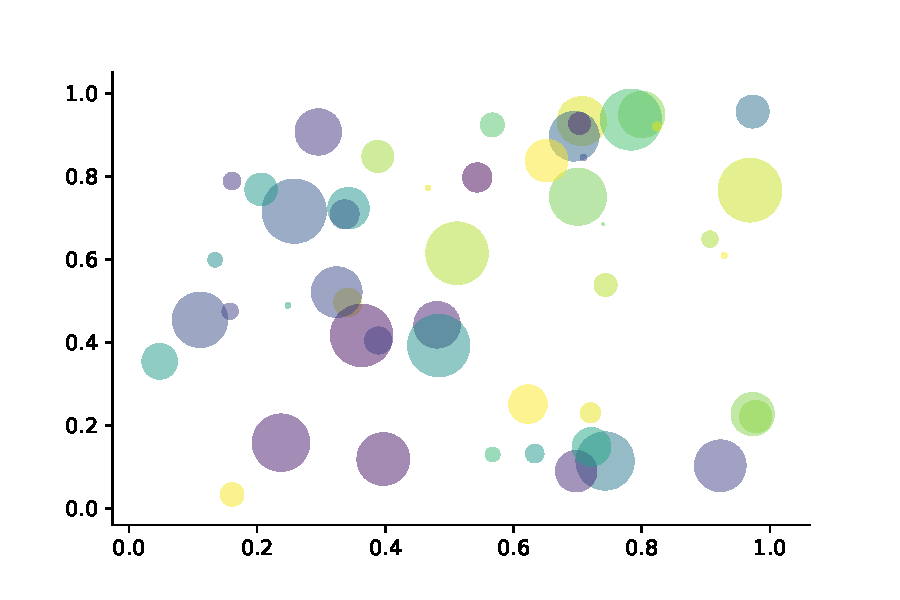
\includegraphics[width=0.6\textwidth]{scatter.pdf}
	\caption{散点图示例 $\hat{y}=a+bx$ \label{fig:scatter}}
\end{figure}

以最简单的一元线性模型来解释最小二乘法。什么是一元线性模型呢?监督学习中,如果预测的变量是离散的,我们称其为分类(如决策树,支持向量机等),如果预测的变量是连续的,我们称其为回归。回归分析中,如果只包括一个自变量和一个因变量,且二者的关系可用一条直线近似表示,这种回归分析称为一元线性回归分析。如果回归分析中包括两个或两个以上的自变量,且因变量和自变量之间是线性关系,则称为多元线性回归分析。对于二维空间线性是一条直线;对于三维空间线性是一个平面,对于多维空间线性是一个超平面。

\begin{property}\label{property:cauchy}
柯西列的性质
\begin{enumerate}
\item $\{x_k\}$ 是柯西列,则其子列 $\{x_k^i\}$ 也是柯西列。
\item $x_k\in \mathcal{R}^n$,$\rho(x,y)$ 是欧几里得空间,则柯西列收敛,$(\mathcal{R}^n,\rho)$ 空间是完备的。
\end{enumerate}
\end{property}

\begin{conclusion}
回归分析(regression analysis) 是确定两种或两种以上变量间相互依赖的定量关系的一种统计分析方法。运用十分广泛,回归分析按照涉及的变量的多少,分为一元回归和多元回归分析;按照因变量的多少,可分为简单回归分析和多重回归分析;按照自变量和因变量之间的关系类型,可分为线性回归分析和非线性回归分析。
\end{conclusion}

\begin{problemset}
\item 设 $A$ 为数域 $K$ 上的 $n$ 级矩阵。证明:如果 $K^n$ 中任意非零列向量都是 $A$ 的特征向量,则 $A$ 一定是数量矩阵。
\item 证明:不为零矩阵的幂零矩阵不能对角化。
\item 设 $A = (a_{ij})$ 是数域 $K$ 上的一个 $n$ 级上三角矩阵,证明:如果 $a_{11} = a_{22} = \cdots = a_{nn}$,并且至少有一个 $a_{kl} \not = 0 (k < l)$,则 $A$ 一定不能对角化。
\end{problemset}

\chapter{常见问题集}

\begin{custom}{问题}
有没有办法章节用“第一章,第一节,(一)”这种?
\end{custom}

\begin{solution}
你可以修改模板中对于章节的设置,利用 ctex 宏集的 \lstinline{\zhnumber} 命令可以把计数器的数字形式转为中文。
\end{solution}


\begin{custom}{问题}
3.07 版本的 cls 的 natbib 加了numbers 编译完了没变化,群主设置了不可更改了?
\end{custom}

\begin{solution}
3.07 中在 \lstinline{gbt7714} 宏包使用时,加入了 \lstinline{authoryear} 选项,这个使得 \lstinline{natbib} 设置了 \lstinline{numbers} 也无法生效。3.08 和 3.09 版本中,模板新增加了 \lstinline{numbers} 、\lstinline{super} 和 \lstinline{authoryear} 文献选项,你可以参考前文设置说明。
\end{solution}

\begin{custom}{问题}
大佬,我想把正文字体改为亮色,背景色改为黑灰色。
\end{custom}

\begin{solution}
页面颜色可以使用 \lstinline{\pagecolor} 命令设置,文本命令可以参考\href{https://tex.stackexchange.com/questions/278544/xcolor-what-is-the-equivalent-of-default-text-color}{这里}进行设置。
\end{solution}

\begin{custom}{问题}
\lstinline[breaklines]{Package ctex Error: CTeX fontset `Mac' is unavailable.}
\end{custom}

\begin{solution}
在 Mac 系统下,中文编译请使用 \lstinline{XeLaTeX}。
\end{solution}

\begin{custom}{问题}
\lstinline{! LaTeX Error: Unknown option `scheme=plain' for package `ctex'.}
\end{custom}

\begin{solution}
你用的 C\TeX{} 套装吧?这个里面的 \lstinline{ctex} 宏包已经是已经是 10 年前的了,与本模板使用的 \lstinline{ctex} 宏集有很大区别。不建议 C\TeX{} 套装了,请卸载并安装 \TeX{} Live 2019。
\end{solution}

\begin{custom}{问题}
我该使用什么版本?
\end{custom}

\begin{solution}
请务必使用\href{https://github.com/ElegantLaTeX/ElegantBook/releases}{最新正式发行版},发行版间不定期可能会有更新(修复 bug 或者改进之类),如果你在使用过程中没有遇到问题,不需要每次更新\href{https://github.com/ElegantLaTeX/ElegantBook/archive/master.zip}{最新版},但是在发行版更新之后,请尽可能使用最新版(发行版)!最新发行版可以在 Github 或者 \TeX{} Live 2019 内获取。
\end{solution}


\begin{custom}{问题}
我该使用什么编辑器?
\end{custom}

\begin{solution}
你可以使用 \TeX{} Live 2019 自带的编辑器 \TeX{}works 或者使用 \TeX{}studio,\TeX works 的自动补全,你可以参考我们的总结 \href{https://github.com/EthanDeng/texworks-autocomplete}{\TeX works 自动补全}。推荐使用 \TeX{} Live 2019 + \TeX Studio。我自己用 VS Code 和 Sublime Text,相关的配置说明,请参考 \href{https://github.com/EthanDeng/vscode-latex}{\LaTeX{} 编译环境配置:Visual Studio Code 配置简介} 和 \href{https://github.com/EthanDeng/sublime-text-latex}{Sublime Text 搭建 \LaTeX{} 编写环境}。
\end{solution}


\begin{custom}{问题}
您好,我们想用您的 ElegantBook 模板写一本书。关于机器学习的教材,希望获得您的授权,谢谢您的宝贵时间。
\end{custom}

\begin{solution}
模板的使用修改都是自由的,你们声明模板来源以及模板地址(github 地址)即可,其他未尽事宜按照开源协议 LPPL-1.3c。做好之后,如果方便的话,可以给我们一个链接,我把你们的教材放在 ElegantLaTeX 用户作品集里。
\end{solution}

\begin{custom}{问题}
我想要原来的封面!
\end{custom}

\begin{solution}
我们计划在未来版本加入封面选择,让用户可以选择旧版封面。
\end{solution}

\begin{custom}{问题}
我想修改中文字体!
\end{custom}

\begin{solution}
首先,我们{\heiti 强烈建议你不要去修改字体}!如果你一定坚持修改字体,请在 \lstinline{newtxtext} 宏包加载前加入中文字体设置(\lstinline{xeCJK} 宏包)。

如果你选择自定义字体,请设置好 \lstinline{\kaishu},\lstinline{\heiti} 等命令,否则会报错。如果你看不懂我现在说的,请停止你的字体自定义行为。
\end{solution}

\begin{custom}{问题}
请问交叉引用是什么?
\end{custom}

\begin{solution}
本群和本模板适合有一定 \LaTeX{} 基础的用户使用,新手请先学习 \LaTeX{} 的基础,理解各种概念,否则你将寸步难行。
\end{solution}

\begin{custom}{问题}
定义等环境中无法使用加粗命令么?
\end{custom}

\begin{solution}
是这样的,默认中文并没加粗命令,如果你想在定义等环境中使用加粗命令,请使用 \lstinline{\heiti} 等字体命令,而不要使用 \lstinline{\textbf}。或者,你可以将 \lstinline{\textbf} 重新定义为 \lstinline{\heiti}。英文模式不存在这个问题。
\end{solution}

\begin{custom}{问题}
代码高亮环境能用其他语言吗?
\end{custom}

\begin{solution}
可以的,ElegantBook 模板用的是 \lstinline{listings} 宏包,你可以在环境(\lstinline{lstlisting})之后加上语言(比如 Python 使用 \lstinline{language=Python} 选项),全局语言修改请使用 \lstinline{\lstset} 命令,更多信息请参考宏包文档。
\end{solution}


\begin{custom}{问题}
群主,什么时候出 Beamer 的模板(主题),ElegantSlide 或者 ElegantBeamer?
\end{custom}

\begin{solution}
这个问题问的人比较多,我这里给个明确的答案。由于 Beamer 中有一个很优秀的主题 \href{https://github.com/matze/mtheme}{Metropolis}。我觉得在我们找到非常好的创意之前不会发布正式的 Beamer 主题,如果你非常希望得到 Elegant\LaTeX{} “官方”的主题,请在用户 QQ 群内下载我们测试主题 PreElegantSlide(未来不一定按照这个制作)。正式版制作计划在 2020 年之后。
\end{solution}


\nocite{*} 

\bibliography{reference}

\appendix
\chapter{基本数学工具}

本附录包括了计量经济学中用到的一些基本数学,我们扼要论述了求和算子的各种性质,研究了线性和某些非线性方程的性质,并复习了比例和百分数。我们还介绍了一些在应用计量经济学中常见的特殊函数,包括二次函数和自然对数,前 4 节只要求基本的代数技巧,第 5 节则对微分学进行了简要回顾;虽然要理解本书的大部分内容,微积分并非必需,但在一些章末附录和第 3 篇某些高深专题中,我们还是用到了微积分。

\section{求和算子与描述统计量}

\textbf{求和算子} 是用以表达多个数求和运算的一个缩略符号,它在统计学和计量经济学分析中扮演着重要作用。如果 $\{x_i: i=1, 2, \ldots, n\}$ 表示 $n$ 个数的一个序列,那么我们就把这 $n$ 个数的和写为:

\begin{equation}
\sum_{i=1}^n x_i \equiv x_1 + x_2 +\cdots + x_n
\end{equation}

\chapter{最小示例}

\begin{lstlisting}
\documentclass[lang=cn,11pt]{elegantbook}
% title info
\title{Title}
\subtitle{Subtitle is here}
% bio info
\author{Your Name}
\institute{XXX University}
\date{\today}
% extra info
\version{1.00}
\extrainfo{Victory won\rq t come to us unless we go to it. --- M. Moore}
\logo{logo.png}
\cover{cover.jpg}

\begin{document}

\maketitle
\tableofcontents
\mainmatter
\hypersetup{pageanchor=true}
% add preface chapter here if needed
\chapter{Example Chapter Title}
The content of chapter one.

\bibliography{reference}

\end{document}
\end{lstlisting}


\end{document}
